

\documentclass[tikz, border=10pt]{standalone}
\documentclass{standalone}
\usepackage{tikz}

\begin{document}

\begin{tikzpicture}[x=1cm, y=1cm] % Adjust the scale as needed
    % Set the width of the number line (adjust as needed)
    \draw[->] (-10,0) -- (10,0);
    
    % Draw tick marks and labels
    \foreach \x/\label in {-10/A, -5/, 0/, 5/, 10/B} {
        \draw (\x,-0.1) -- (\x,0.1);
        \node[below] at (\x,-0.2) {\label};
    }
\end{tikzpicture}
\\
zzzzz

% \documentclass[tikz, border=10pt]{standalone}
% \usepackage{tikz}

\begin{document}
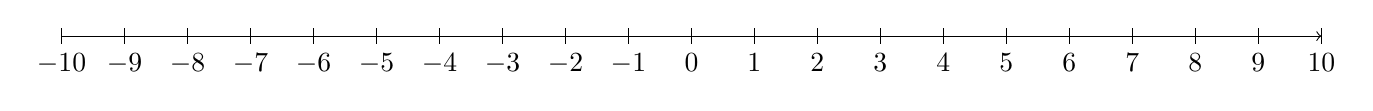
\begin{tikzpicture}[x=0.8cm]
    % Draw the main line
    \draw[->] (-10,0) -- (10,0);
    
    % Draw tick marks and labels
    \foreach \x in {-10, -9, ..., 10} {
        \draw (\x,-0.1) -- (\x,0.1) node[below, yshift=-2mm] {$\x$};
    }
\end{tikzpicture}
%\end{document}

zzzzz
\\

 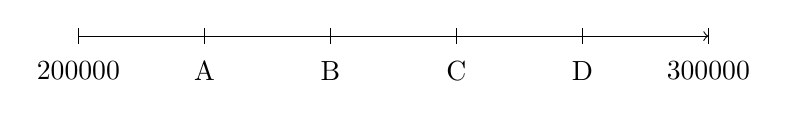
\begin{tikzpicture}[x=0.8cm]
    % Draw the main line
    \draw[->] (0,0) -- (10,0);
    
    % Draw tick marks and labels
    \foreach \x/\label in {0/200000, 2/220000, 4/240000, 6/260000, 8/280000, 10/300000} {
        \draw (\x,-0.1) -- (\x,0.1);
        % Omit labels at positions 4 and 8 to leave them blank
        \ifnum\x=2 \else \ifnum\x=4 \else \ifnum\x=6 \else \ifnum\x=8 \else
            \node[below] at (\x,-0.2) {\label};
        \fi\fi\fi\fi
    }
    
    % Draw letters 'X' and 'Y' at positions 4 and 8
    \node[below] at (2,-0.2) {A};
    \node[below] at (4,-0.2) {B};
    \node[below] at (6,-0.2) {C};
    \node[below] at (8,-0.2) {D};
    
\end{tikzpicture}
\vspace{10pt}

%Trying 1

 \begin{tikzpicture}[x=0.8cm]
    % Draw the main line
    \draw[->] (-15,0) -- (10,0);
    
    % Draw tick marks and labels
    \foreach \x/\label in {-15/-15, -10/-10, -5/-5, 0/0, 5/5, 10/10} {
        \draw (\x,-0.1) -- (\x,0.1);
        % Omit labels at positions 4 and 8 to leave them blank
        \ifnum\x=-10 \else \ifnum\x=-5 \else \ifnum\x=5 \else
            \node[below] at (\x,-0.2) {\label};
        \fi\fi\fi
    }
    
    % Draw letters 'X' and 'Y' at positions 4 and 8
    \node[below] at (-10,-0.2) {A};
    \node[below] at (-5,-0.2) {B};
    \node[below] at (5,-0.2) {C};
    % \node[below] at (8,-0.2) {D};
    
\end{tikzpicture}
\\
\vspace{10pt}

%\documentclass[tikz, border=10pt]{standalone}
%\usepackage{tikz}

%\begin{document}
Working Try 2 (70\% ) 
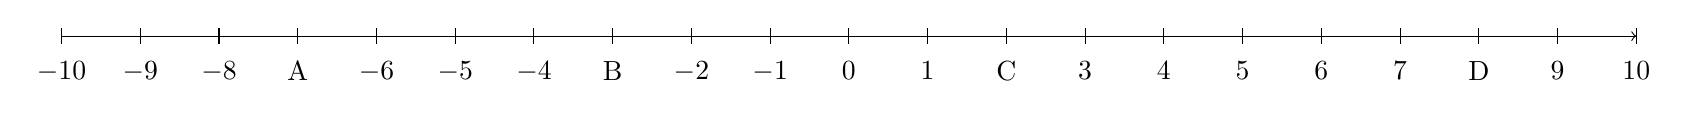
\begin{tikzpicture}[x=1cm]  % Set the x unit vector length to 1cm
    % Draw the main line
    \draw[->] (-10,0) -- (10,0);
    
    % Draw tick marks and labels
    \foreach \x in {-10, -9, ..., 10} {
        \draw (\x,-0.1) -- (\x,0.1);
        % Omit labels at positions -7, -3, 2, and 8 to leave them blank for letters
        \ifnum\x=-7 \else \ifnum\x=-3 \else \ifnum\x=2 \else \ifnum\x=8 \else
            \node[below] at (\x,-0.2) {$\x$};
        \fi\fi\fi\fi
    }
    
    % Draw letters 'A', 'B', 'C', and 'D' at positions -7, -3, 2, and 8
    \node[below] at (-7,-0.2) {A};
    \node[below] at (-3,-0.2) {B};
    \node[below] at (2,-0.2) {C};
    \node[below] at (8,-0.2) {D};
    
\end{tikzpicture}

\text{Working} 
Try 3

\begin{tikzpicture}[x=0.8cm]  % Set the x unit vector length to 
    % Draw the main line
    \draw[->] (-10,0) -- (10,0);
    
    % Draw tick marks and labels
    \foreach \x in {-10, -5, ..., 10} {
        \draw (\x,-0.1) -- (\x,0.1);
        % Omit labels at positions -7, -3, 2, and 8 to leave them blank for letters
        \ifnum\x=-5 \else \ifnum\x=0 \else \ifnum\x=5 \else 
            \node[below] at (\x,-0.2) {$\x$};
        \fi\fi\fi
    }
    
    % Draw letters 'A', 'B', 'C', and 'D' at positions -7, -3, 2, and 8
    \node[below] at (-5,-0.2) {A};
    \node[below] at (0,-0.2) {B};
    \node[below] at (5,-0.2) {C};
    %\node[below] at (8,-0.2) {D};
    
\end{tikzpicture}
\\
\vspace{10pt}

Try 4 
\begin{tikzpicture}[x=0.8cm]  % Set the x unit vector length to 
    % Draw the main line
    \draw[->] (-10,0) -- (10,0);
    
    % Draw tick marks and labels
    \foreach \x in {-10, -8, ..., 10} {
        \draw (\x,-0.1) -- (\x,0.1);
        % Omit labels at positions -7, -3, 2, and 8 to leave them blank for letters
        \ifnum\x=-8 \else \ifnum\x=-6 \else \ifnum\x=-4 \else \ifnum\x=-2 \else 
        \ifnum\x=2 \else \ifnum\x=4 \else \ifnum\x=6 \else \ifnum\x=8 \else 
            \node[below] at (\x,-0.2) {$\x$};
        \fi\fi\fi\fi\fi\fi\fi\fi
    }
    
    % Draw letters 'A', 'B', 'C', and 'D' at positions -7, -3, 2, and 8
    \node[below] at (-8,-0.2) {A};
    \node[below] at (-2,-0.2) {B};
    \node[below] at (4,-0.2) {C};
    \node[below] at (8,-0.2) {D};
    
\end{tikzpicture}

\vspace{10pt}

% \( \displaystyle \frac{\partial Q}{\partial t} = \frac{\partial s}{\partial t} \)

\( P(\neg A)  \)


\end{document}
